\chapter{Example: conformal maps of surfaces}%
\label{chapter:conformal.maps}%
\chapterSummary{We use the Cartan--K\"ahler theorem to prove the existence of local conformal maps between surfaces. We assume familiarity with appendix~\ref{chapter:moving.frame}.}%
\section{Conformal maps}A \emph{conformal map}\define{conformal} is a local diffeomorphism \(\phi \colon S \to \ot{S}\) between surfaces in \(\E[3]\) preserving angles between curves.
\begin{center}
\includegraphics[height=4cm]{earth.jpg}
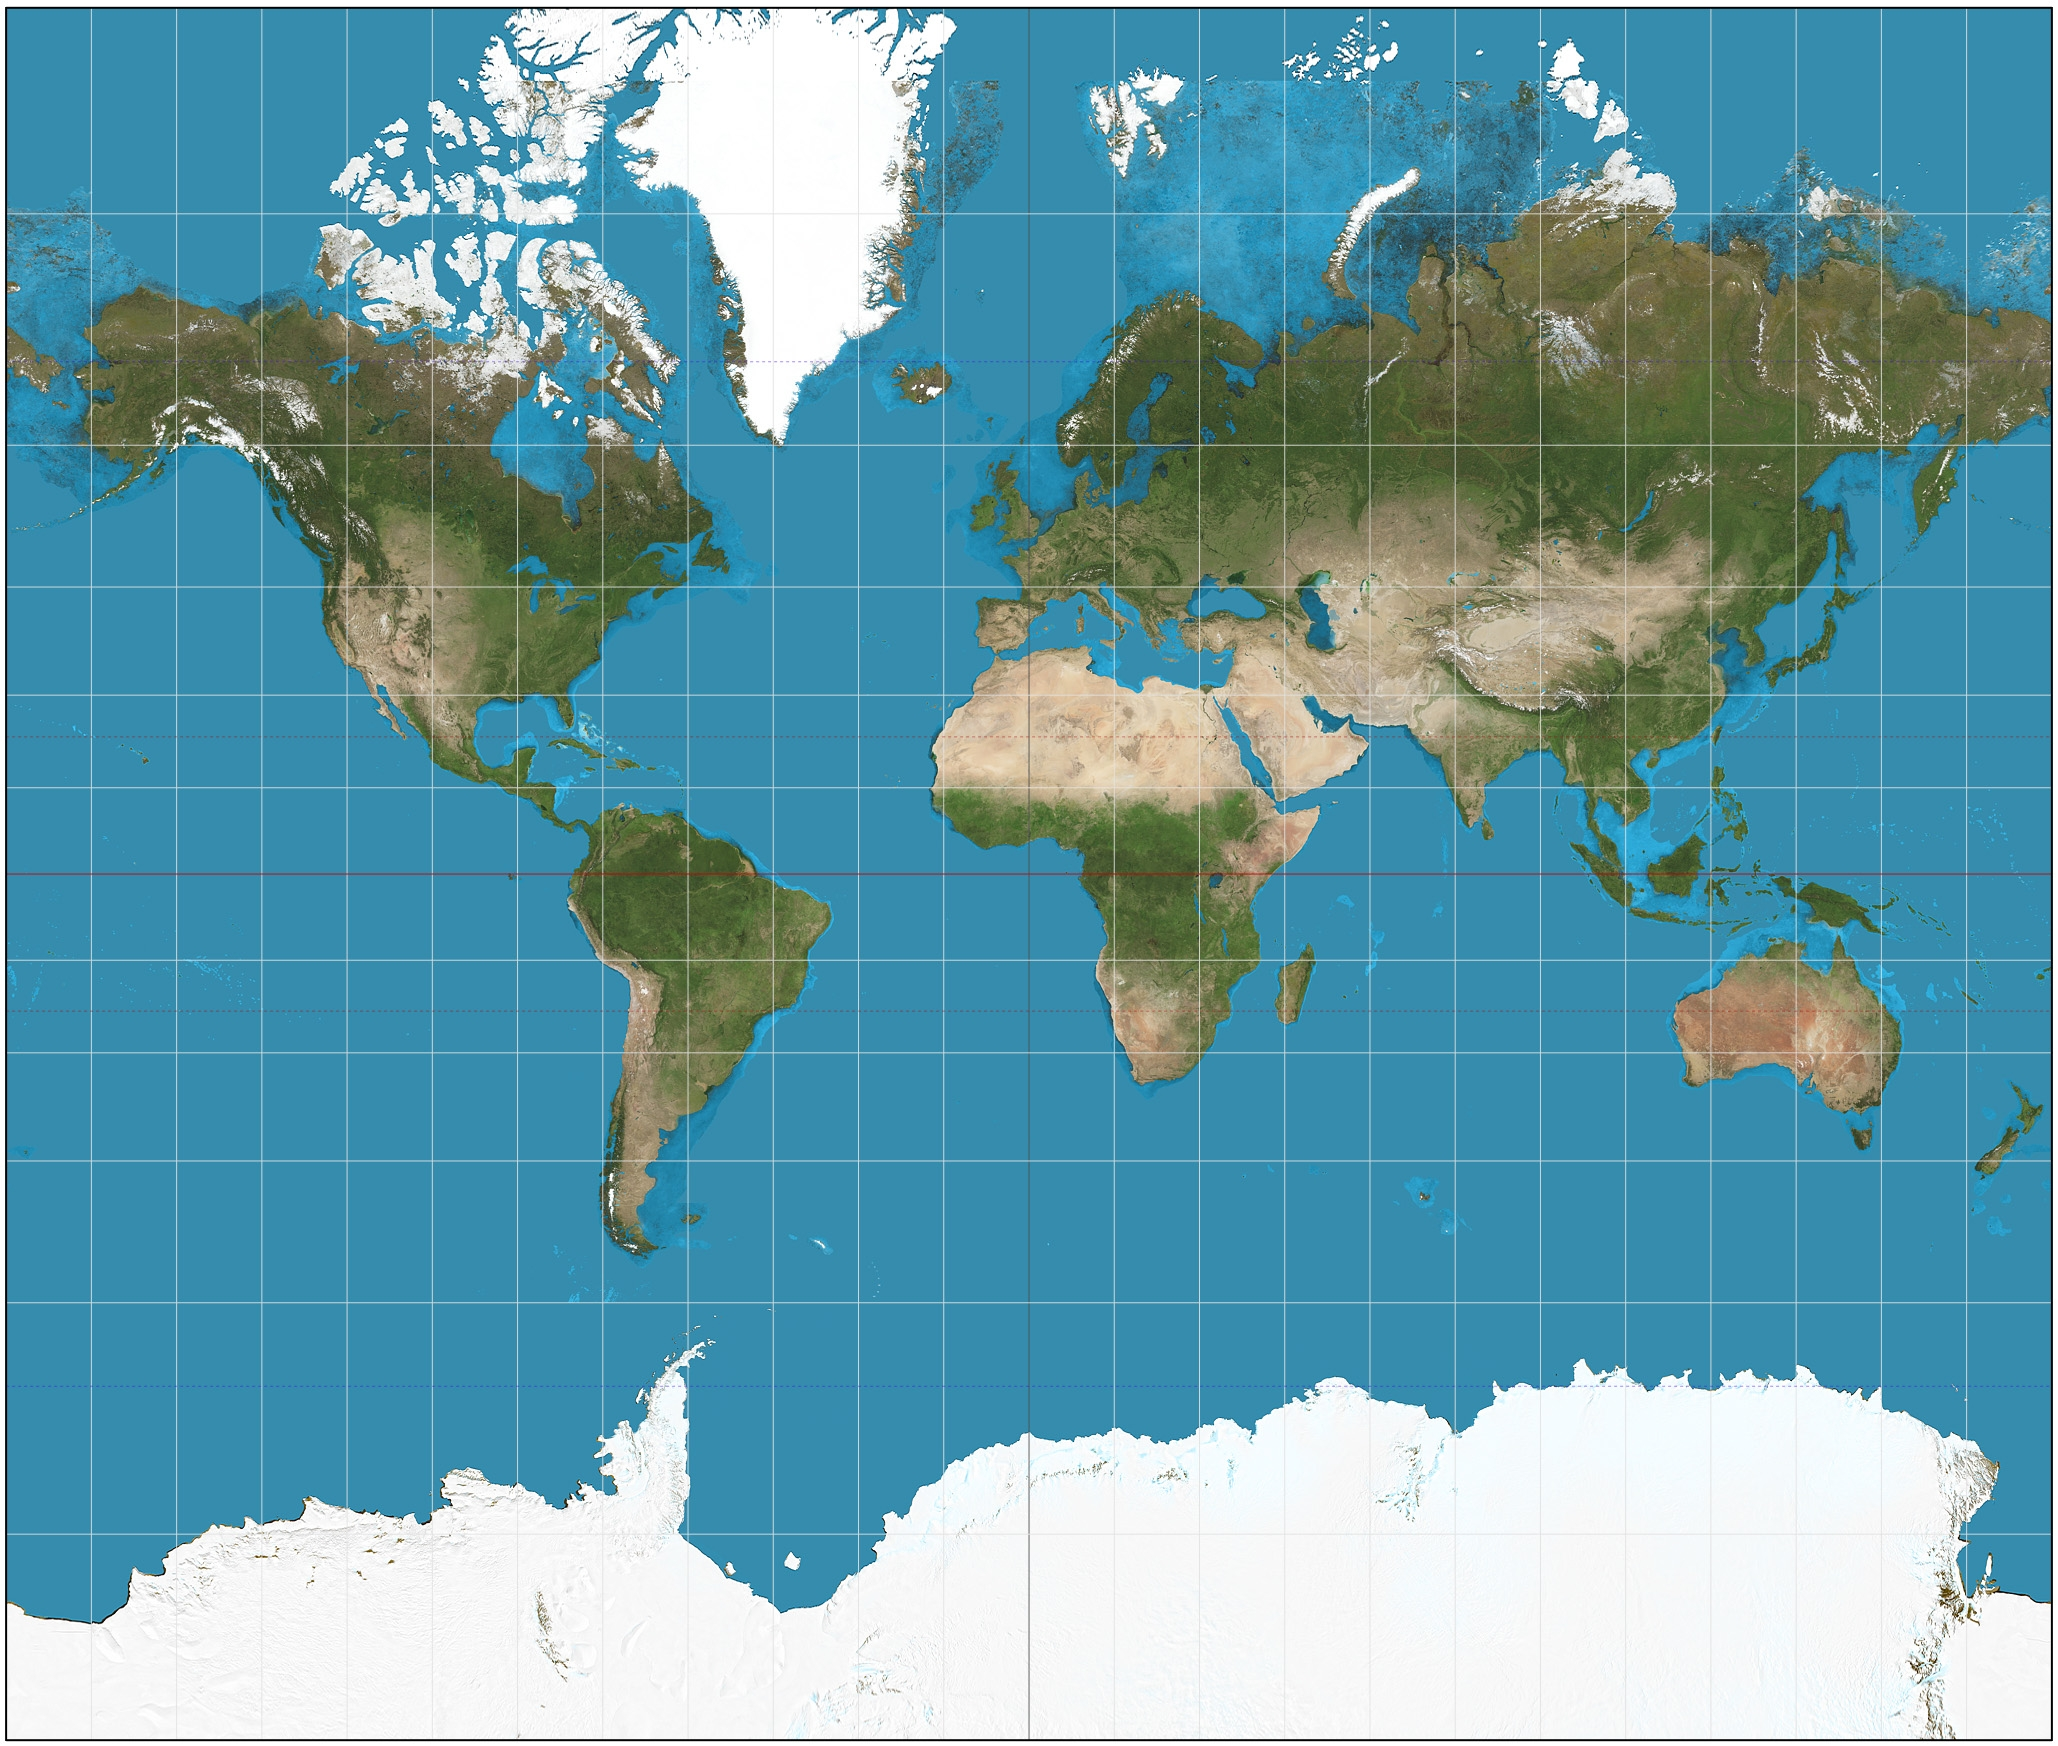
\includegraphics[height=4cm]{Mercator_projection_SW.jpg}
{\tiny
\smallskip\par
\begin{minipage}{8cm}
Mercator projection, a conformal map of an open subset of the sphere. 
\par\noindent
By Strebe - Own work, CC BY-SA 3.0,
\par\noindent
\url{https://commons.wikimedia.org/w/index.php?curid=16115307!}
\end{minipage}}
\end{center}
\begin{theorem}
Given two surfaces \(S, \ot{S}\) in \(\E[3]\), and points \(x_0 \in S, \ot{x}_0 \in \ot{S}\), there is a conformal map \(\phi \colon U \to \ot{U}\) from an open set \(U \subset S\) containing \(x_0\) to an open set \(\ot{U} \subset \ot{S}\) containing \(\ot{x}_0\) so that \(\phi\of{x_0}=\ot{x}_0\).
\end{theorem}
See \cite{Douady/Buff:2000} for an elementary proof for smooth surfaces.
\begin{problem}{apply.eds:conformal}
Prove that a linear isomorphism of the plane preserves angles just it is uniquely expressed as a product of a rotation, a rescaling, and perhaps a reflection:
\[
r
\begin{pmatrix}
\cos \theta & -\sin \theta\\
\sin \theta & \cos \theta
\end{pmatrix}
\]
or
\[
r
\begin{pmatrix}
\cos \theta & -\sin \theta\\
\sin \theta & \cos \theta
\end{pmatrix}
\begin{pmatrix}
1 & 0\\
0 & -1
\end{pmatrix}.
\]
\end{problem}
\begin{problem}{apply.eds:conformal.rotation}
Given two surfaces of revolution, show that we can explicitly compute a rotationally invariant conformal map from one to the other by solving a first order ordinary differential equation for one function of one variable.
If one of the surfaces is a cylinder or a sphere, explain how to reduce the construction of the conformal map to solving an integral, rather than an ordinary differential equation.
\end{problem}
\section{The graph of a conformal map as an integral manifold}
It is convenient to write the conformal scaling factor not as \(r\) but instead as \(e^{-u}\).
Suppose that \(\phi \colon S \to \ot{S}\) is a conformal map.
Inside the \(7\)-dimensional manifold \(M\defeq\frameBundle{S} \times \frameBundle{\ot{S}} \times \R_u\), consider the \(3\)-dimensional submanifold \(X\) consisting of points \((x,e,\ot{x},\ot{e},u)\) with \((x,e) \in \frameBundle{S}\) and \(\pr{\ot{x},\ot{e}}\in \frameBundle{\ot{S}}\) so that
\begin{align*}
\ot{x}&=\phi(x), \\
\ot{e}_1&=e^{-u} \phi'(x)e_1, \\
\ot{e}_2&=e^{-u} \phi'(x)e_2.
\end{align*}
Recall the structure equations \(d\omega=i\alpha\wedge\omega\) on \(S\) and \(d\otomega=i\otalpha\wedge\otomega\) on \(\ot{S}\).
\begin{problem}{apply.eds:omegas}
On \(X\), show that \(\otomega=e^{-u}\omega\) and  \(du+i(\otalpha-\alpha)=u'\omega\) for a unique function \(u'\) on \(X\).
\end{problem}
\begin{answer}{apply.eds:omegas}
\begin{align*}
\otomega_1
&=
\ot{e}_1 \cdot d\ot{x},
\\
&=
e^{-u} \pr{\phi'(x) e_1} \cdot d\phi(x),
\\
&=
e^{-u} \pr{\phi'(x) e_1} \cdot \phi'(x) \, dx,
\\
&=
e^{-u} e_1 \cdot dx,
\\
&=
e^{-u} \omega_1, 
\end{align*}
and similarly \(\otomega_2=e^{-u} \omega_2\).
So \(\otomega=e^{-u}\omega\).
Differentiate to get 
\[
d\otomega = i\otalpha\wedge\otomega=d(e^{-u}\omega),
\]
which we expand out to find
\[
(du+i(\otalpha-\alpha)\wedge\otomega=0.
\]
By the complex linear form of Cartan's lemma (which the reader can state and prove), we get the result.
\end{answer}
On the \(7\)-dimensional manifold \(M\), take the exterior differential system \(\II\) generated by \(\otomega - e^{-u} \omega\).
Any conformal map \(\phi \colon S \to \ot{S}\) has associated submanifold \(X\) of \(\frameBundle{S} \times \frameBundle{\ot{S}}\) an integral manifold.
The tableau is
\[
d(\otomega-e^{-u}\omega)
=
e^{-u}(du+i(\otalpha-\alpha))\wedge\omega.
\]
In real and imaginary parts, the tableau \(du+i(\otalpha-\alpha)\) is
\[
\Tablo{*du,-(\otalpha-\alpha);*\otalpha-\alpha,du}[2,0]
%\begin{pmatrix}
%\freeDeriv{du} & -(\otalpha-\alpha)\\
%\freeDeriv{\otalpha-\alpha} & du
%\end{pmatrix}
\]
%with characters \(s_1,s_2=2,0\). 
The integral elements are the complex numbers \(u'\) so that \(du+i(\otalpha-\alpha)=u'\omega\), i.e. the real and imaginary parts of these numbers, \(s_1+2s_2=2+2(0)=2=s\), involution: an integral manifold \(X \subset M\) exists through any point of \(M\).

Finally, we need to prove that our integral manifold is actually constructed from some conformal map \(\phi\).
Since \(u\) is real, \(du+i(\otalpha-\alpha)\) has real part \(du\) and imaginary part \(\otalpha-\alpha\).
Note that \(\II\) has a Cauchy characteristic: the vector fields \(v\) on which \(\alpha \ne 0\) but 
\[
0=\omega_1=\omega_2=\otomega_1=\otomega_2=du=\otalpha-\alpha.
\]
We can in addition quotient by a reflection \(e_2\mapsto -e_2, \ot{e}_2\mapsto -\ot{e}_2\).
The quotient space \(\bar{M}\) is the set of all conformal linear maps from tangent spaces of \(S\) to those of \(\ot{S}\), as we are quotienting out by conformally changing the frame \(e_1, e_2\) and correspondingly the frame \(\ot{e}_1, \ot{e}_2\).
So \(\bar{M}\) is a \(3\)-manifold, and \(X\) projects to a surface \(\bar{X}\) in \(\bar{M}\).
As \(\omega_1, \omega_2, \alpha\) are linearly independent on \(X\), \(\bar{X}\) has \(\omega_1, \omega_2\) still linearly independent, since both \(\omega_1\) and \(\omega_2\) vanish on the Cauchy characteristic vectors.
Therefore \(\bar{X}\) projects to \(S\) by a local diffeomorphism.
Similarly, \(\bar{X}\) projects to \(\ot{S}\) by a local diffeomorphism.
So \(\bar{X}\) injects into \(S \times \ot{S}\), as the graph of a local diffeomorphism, say \(\phi \colon S \to \ot{S}\). 

We need to prove that \(\phi\) is conformal.
Take some tangent vector \(v \in T_x S\).
Pick a point 
\[
\pr{x,e,\ot{x},\ot{e}} \in X.
\]
Write the vector \(v\) as \(v=v_1 e_1 + v_2 e_2\).
We make a vector \(\hat{v}\) on \(X\) which projects to \(v\), by asking that
\[
\hat{v} \hook 
\begin{pmatrix}
\omega_1 \\
\omega_2 \\
\alpha
\end{pmatrix}
=
\begin{pmatrix}
v_1 \\
v_2 \\
0
\end{pmatrix}.
\]
Then \(\hat{v}\) projects to \(\ot{S}\) to a vector \(\ot{v}\) with \(\ot{v}=\ot{v}_1 \ot{e}_1 + \ot{v}_2 \ot{e}_2\) given by
\[
\hat{v} \hook 
\begin{pmatrix}
\otomega_1 \\
\otomega_2
\end{pmatrix}
=
\begin{pmatrix}
\ot{v}_1 \\
\ot{v}_2
\end{pmatrix}.
\]
But on \(X\), \(\otomega_1=e^{-u}\omega_1\), \(\otomega_2=e^{-u}\omega_2\) so
\[
\begin{pmatrix}
\ot{v}_1 \\
\ot{v}_2
\end{pmatrix}
= 
e^{-u}
\begin{pmatrix}
v_1 \\
v_2
\end{pmatrix}.
\]
In other words, \(\ot{v}=e^{-u}v_1 \ot{e}_1 + e^{-u}v_2 \ot{e}_2\), so that \(\phi\) is a conformal map.

\section{Characteristics}
\begin{theorem}
Take any two surfaces \(S, \ot{S}\) in \(\E[3]\), and embedded curves \(C \subset S\) and \(\ot{C} \subset \ot{S}\).
Every local diffeomorphism \(\phi \colon C \to \ot{C}\) extends to a conformal map \(\phi \colon U \to \ot{U}\) from an open set \(U \subset S\) containing \(C\) to an open set \(\ot{U} \subset \ot{S}\) containing \(\ot{C}\).
Any two such maps agree on any connected open neighborhood of \(C\) on which both are defined.
\end{theorem}
Note that the curves \(C, \ot{C}\) may be closed curves here; the result is global as regards the curves, but local in that we only construct a conformal map near the curves.
\begin{example}
Near each point of any surface, there is a conformal map to the plane, i.e. there are coordinates \(x,y\), called \emph{isothermal},\define{isothermal coordinates}\define{coordinates!isothermal} identifying angle measurements with those of the plane
\end{example}
\begin{proof}
The characteristic variety of our tableau:
\[
\Tablo{*\pi^1,-\pi^2;*\pi^2,\pi^1}
=
\Tablo{*du,-(\otalpha-\alpha);*\otalpha-\alpha,du}
\]
Replace each polar \(\pi^{\alpha}\) in the tableau with \(v^{\alpha}\xi\):
\[
0=
\begin{tableau}
v^1\xi & v^2\xi \\
-v^2\xi & v^1\xi
\end{tableau}
\wedge
\begin{pmatrix}
\omega^1\\
\omega^2
\end{pmatrix}
=
\begin{pmatrix}
v^2\xi_1-v^1\xi_2\\
v^1\xi_1+v^2\xi_2
\end{pmatrix}
\omega^{12}
=
\begin{pmatrix}
-\xi_2 & \xi_1 \\
\xi_1 & \xi_2
\end{pmatrix}
\begin{pmatrix}
v^1\\
v^2
\end{pmatrix}
\omega^{12}.
\]
The characteristic variety equation is the determinant of the symbol matrix: \(\xi_1^2+\xi_2^2=0\), i.e. there are no real characteristics, an elliptic determined system after we mod out the Cauchy characteristics.
So any integral curve in \(\bar{M}\) lies in a unique integral surface.
A curve in the \(6\)-dimensional manifold \(\bar{M}\) is a choice of curve \(C\) in \(S\), a curve \(\ot{C}\) in \(\ot{S}\), a diffeomorphism between the curves, and a conformal factor \(e^{-u}\) along the curve.
Such a curve is an integral curve of the system just when \(\otomega_i=e^{-u}\omega_i\), i.e. \(u\) is determined by the ratio of the lengths of the tangent vector to \(C\) and that to \(\ot{C}\).
\end{proof}